\chapter{User Manual}
Welcome to the User Manual of \texttt{theraleap}, a proof of concept implementation of a computer aided ergotherapy platform. With this Software, you will be able to play Games by performing Gestures with your hand. This Manual will help you to get started!
\section{Getting started}
Please complete these steps in order to get started.
\subsection{Get Chrome}
You will need a recent Version of Chrome. Firefox will not work unfortunately because it will not allow us to talk with the Hand Tracking Device due to Security Restrictions. To get Chrome, visit \url{https://www.google.com/chrome/}
\subsection{Install the Leap Motion Driver}
Currently, we support only the Leap Motion Device for tracking your hand, though that may change in the Future! In order for us to be able to talk to the Leap Motion Device, you'll have to install the Driver. To get the Driver, visit \url{https://developer.leapmotion.com/sdk/v2} and follow the instructions for your Operating System.
\subsection{Try it out}
Now, after everything is installed, and the Device is plugged in, you're ready to test if everything works! Open up Chrome and visit \url{https://talkdirty.github.io/theraleap/#/debug/status}. If all boxes are green, you're ready! If not, follow the instructions you see on screen (it may also take a while for the Leap Motion Device to get ready, so be patient!).

\section{A brief Overview}
\begin{figure}[h]
    \centering
    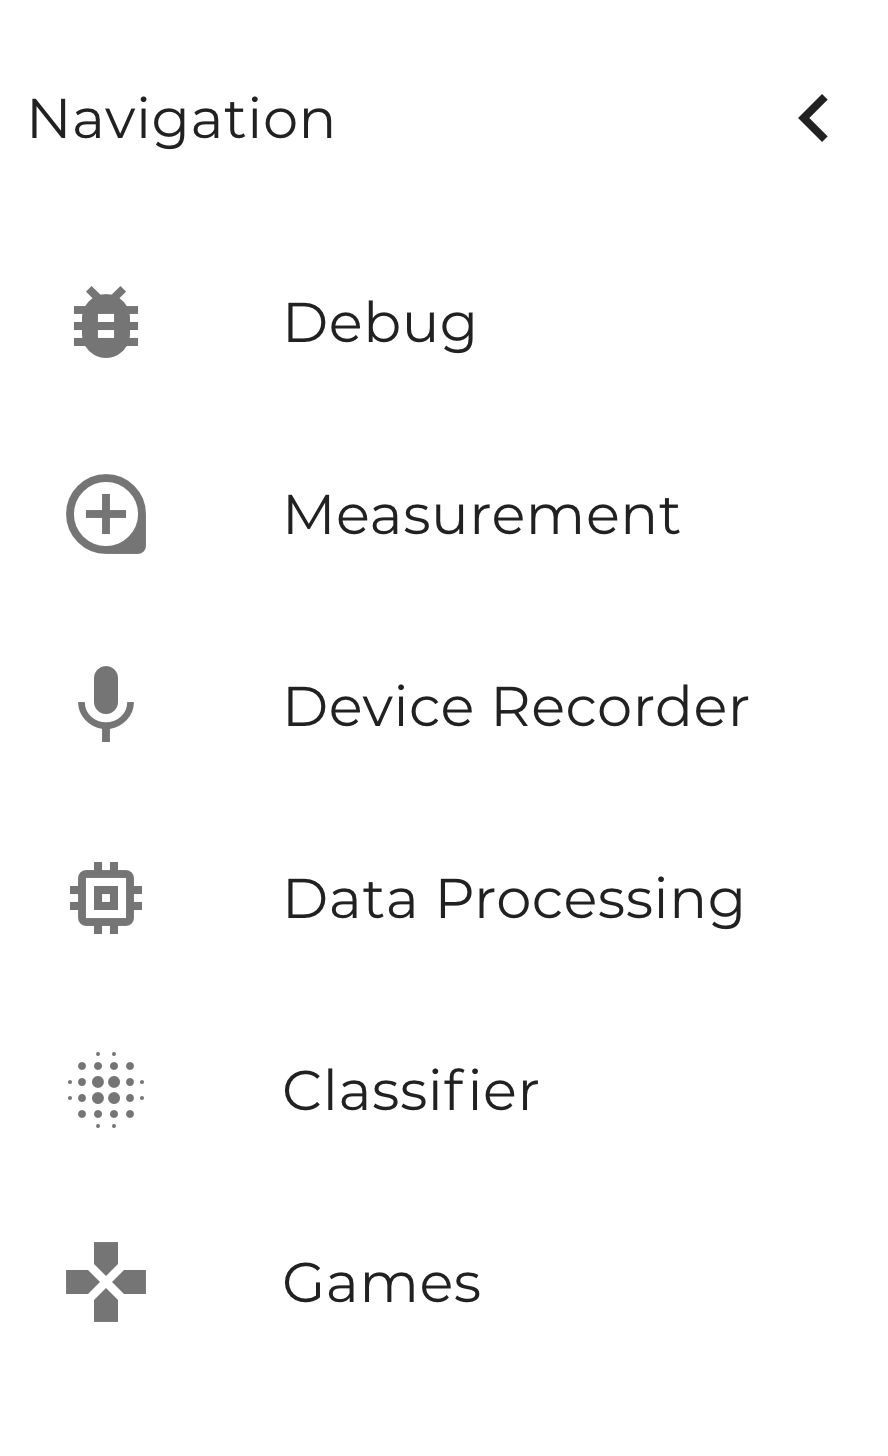
\includegraphics[width=6cm]{navigation}
    \caption{All Navigation Options of the Software}
    \label{fig:navigation}
\end{figure}
You can press the Button on the top left corner to get the Navigation Bar as shown in Figure \ref{fig:navigation}. From here, you can navigate to all available Subcomponents of the Software.

\subsection{Debug}
This is a section containing Information useful to Developers. You can look at the Data coming from the Device, or a graphical representation of your hand here. You probably won't need to spend too much time here though.

\subsection{Measurement}
Here, you can take the angular measurements between your Fingers, a piece of Information required by the Therapist. In order for the measurement to become more accurate, you can choose to average it over several milliseconds, by putting your desired value in the Input Box. On the left hand side, you will see your hand as the Computer sees it. Make sure it is fully visible and is displaying everything correctly. If something is wrong, and the measurement can't be taken, you will be notified of what you need to do in order to fix the problem on the right side of the screen.

\subsection{Device Recorder}
With this Component, you can record your Hand, and play that Data back to the Framework as if it was coming from the real device. As a User of the System, you probably won't ever need this, but this Component is useful for Developers. To start a new Recording, click the \texttt{+} Button. Now you can title your Recording. You also see a miniature Hand on the right side, if you have your hand above the sensor. Once you're ready, press the \texttt{Record} Button. A progress bar will begin to fill, indicating how much space is left for your recording, once it is full, or you press the \texttt{Save} Button, your recording is done. Now you can flip the Switch to activate it. It will then be propagated through the whole System in an endless loop.

If you want to save the Recordings for a later time, make sure the \texttt{Persist Recordings} Checkbox in the Settings Tab is checked.

\subsection{Data Processing}
If your Computer experiences performance issues while working with the System, you can attempt to alleviate this a bit here. Each of the Box shown here is representing a specific preprocessing step. For example, you can limit the framerate of the Device to a lower value such as \texttt{28 FPS} by turning on the \texttt{Limit FPS} Preprocessor. Your system has to do less that way, which will result in a better performance.

\subsection{Classifier}
Here, the Gesture you need to perform in order to control the Games is configured. Each Box represents one specific Gestures. Only one Box can be turned on at a time. Inside the Box, you will find a description of what to do in order to trigger the Gesture, and also some Input Boxes that allow the therapist to configure the Exercise to your needs. He or she might tell you which numbers you should put in here if you train from home.

\subsection{Games}
Finally, here you can choose and play any Game you like. If the Leap Motion Device is attached correctly to your computer, \textbf{and} you turned on a Gesture Classifier in the \texttt{Classifier} Tab, the Button \texttt{Play with Motion Tracking} will be green. Click on it to start the Game. In the game, you can hit \texttt{Space} to Pause or \texttt{Esc} to Quit if you feel tired. Good luck!
